\documentclass{article}
\usepackage{amssymb}
\usepackage{graphicx} 
\usepackage{amsmath}
\usepackage{amsfonts}

\title{Lista 2 Fundamentos Matemáticos da Computação II - Respostas}

\begin{document}

\maketitle

\section{Seção Múltipla Escolha}

\subsection{Questão M1} 
Como $A = \{x \in \mathbb{Z} | 1 \leq x \leq 3\}$ e $B = \{y \in \mathbb{Z} | y \text{ é par e } 0 \leq y \leq 2\}$, logo $A = \{1,2,3\}$ e $B = \{0,2\}$ e o produto cartesiano será:

\[
    A \times B = \{(1,0),(1,2),(2,0),(2,2),(3,0),(3,2)\}
\]

Dessa forma, a alternativa correta é a letra \textbf{C}


\subsection{Questão M2}
% SUA RESPOSTA DA M2
\subsection{Questão M3}
Seja \( A \) um conjunto com cardinalidade \( |A| = 4 \) e \( B \) um conjunto com cardinalidade \( |B| = 3 \). A quantidade de relações binárias distintas entre \( A \) e \( B \) pode ser determinada da seguinte forma:

Uma relação binária entre \( A \) e \( B \) é um subconjunto do produto cartesiano \( A \times B \). O número de elementos do produto cartesiano \( A \times B \) é dado por:

\[
|A \times B| = |A| \times |B| = 4 \times 3 = 12
\]

Agora, como cada elemento de \( A \times B \) pode ser incluído ou não em uma relação, o número total de relações binárias (subconjuntos) s é dado por:

\[
\text{Número de relações binárias} = 2^{12}
\]

Portanto, a alternativa correta é a letra \textbf{B}
\subsection{Questão M4}

Considerando as definições de Injetividade, Sobrejetividade e Bijetividade, a resposta correta é a letra \textbf{E (i) bijetora (ii) injetora (iii) sobrejetora}


\vspace{0.5em}
\hrule
\vspace{0.5em}

\section{Seção Discursiva}

\subsection{Questão D1}
% SUA RESPOSTA DA D1
\subsection{Questão D2}
\begin{figure}[h]
    \centering
    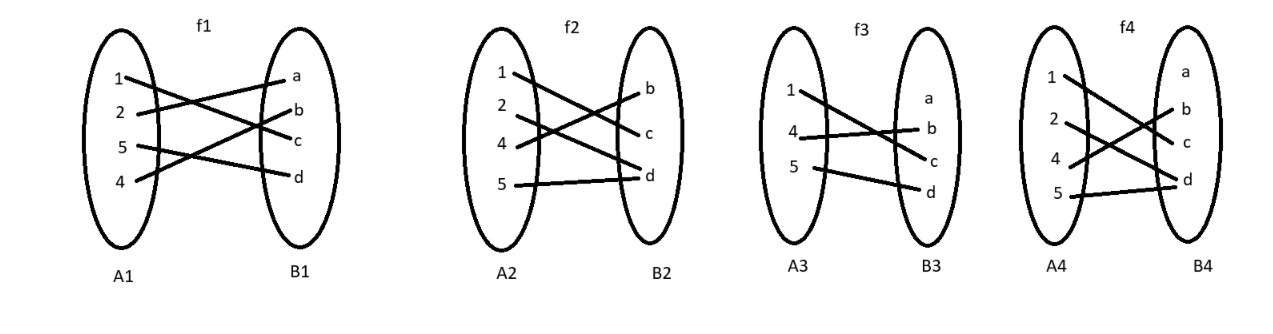
\includegraphics[width=0.8\textwidth]{qd2.png} 
    \label{fig:questaoD2}
\end{figure}
\section*{Análise de Funções}

Dada a relação entre os conjuntos \(A\) e \(B\) para as funções \(f_1, f_2, f_3, f_4\), analisamos se são injetoras, sobrejetoras ou bijetoras:

\begin{itemize}
    \item \textbf{\(f_1\):}
    \begin{itemize}
        \item Cada elemento de \(A1\) tem uma correspondência distinta em \(B1\).
        \item Todos os elementos de \(B1\) são atingidos.
        \item \textbf{Conclusão:} \(f_1\) é \textbf{bijetora} (injetora e sobrejetora).
    \end{itemize}
    \item \textbf{\(f_2\):}
    \begin{itemize}
        \item Nem todos os elementos de \(A2\) possuem imagens distintas (\(2\) e \(5\) têm a mesma imagem em \(B3\)).
        \item Nem todos os elementos de \(B2\) são atingidos (\(a\) não é imagem de nenhum elemento de \(A2\)).
        \item \textbf{Conclusão:} \(f_2\) é \textbf{sobrejetora}.
    \end{itemize}
    \item \textbf{\(f_3\):}
    \begin{itemize}
        \item Cada elemento de \(A3\) tem uma correspondência distinta em \(B3\).
        \item Nem todos os elementos de \(B3\) são atingidos.
        \item \textbf{Conclusão:} \(f_3\) é \textbf{injetora}.
    \end{itemize}
    \item \textbf{\(f_4\):}
    \begin{itemize}
        \item Nem todos os elementos de \(A4\) possuem imagens distintas (\(2\) e \(5\) têm a mesma imagem em \(B4\)).
        \item Nem todos os elementos de \(B4\) são atingidos (\(a\) não é imagem de nenhum elemento de \(A4\)).
        \item \textbf{Conclusão:} \(f_4\) é \textbf{nenhum}.
    \end{itemize}
\end{itemize}


\end{document}
